\documentclass[12pt]{report}
\usepackage{graphicx}
\usepackage{float}
\usepackage{geometry}
\geometry{a4paper, margin=1in}

\usepackage[utf8]{inputenc}
\usepackage[T1]{fontenc}
\usepackage{tikz}
\usetikzlibrary{arrows.meta,positioning,shapes.geometric}

\usepackage{algorithm}
\usepackage{algorithmic}
\usepackage{amsmath}
\usepackage{lmodern}
\usepackage{titlesec}
\titleformat{\chapter}[hang]{\normalfont\Huge\bfseries}{\thechapter.}{1em}{}

\usepackage{setspace}
\usepackage{url}
\usepackage[hidelinks]{hyperref}
\hypersetup{colorlinks=true, linkcolor=black, citecolor=black, urlcolor=blue}

\sloppy
\setstretch{1.4}

\begin{document}

\begin{titlepage}
    \begin{center}
        \vspace*{0.4cm}
        {\Large \textbf{Comparison of Lightweight Encryption Algorithms}}\\[0.3cm]

        {\large A comparative study of secure and efficient cryptographic primitives\\
        for resource-constrained embedded systems}\\[1.0cm]

        \textbf{Technical Writing Report Submitted}\\
        In partial fulfillment of the requirements for the award of the\\
        \textbf{Bachelor of Technology}\\[1.0cm]
        {\large \textbf{Authors}}\\[0.25cm]

        \begin{tabular}{ll}
            \textbf{Rajesh Kumar Jena} & (B122088) \\
            \textbf{Soumil Kumar}      & (B122114) \\
            \textbf{Punit Kumar}       & (B422041)
        \end{tabular}\\[1.0cm]

        {\large \textbf{Under the supervision of}}\\[0.2cm]
        {\textbf{Prof. Debasish Jena}}\\[1.0cm]

        
\includegraphics[width=0.22\textwidth]{iiit-bh-logo.png}\\[0.4cm]
        {\large International Institute of Information Technology, Bhubaneswar}\\[0.15cm]
        {\large November 2025}

    \end{center}
\end{titlepage}

\newpage
\chapter*{Approval of the Viva-Voice Board}
\addcontentsline{toc}{chapter}{Approval of the Viva-Voice Board}
\vspace{1cm}
\noindent November 18, 2025

\vspace{1cm}

\noindent Certified that the report entitled ``Comparison of Lightweight Encryption Algorithms,''
submitted by Rajesh Kumar Jena (B122088), Soumil Kumar (B122114), and Punit Kumar (B422041)
to the International Institute of Information Technology, Bhubaneswar, in partial fulfillment
of the Technical Writing requirements for the award of the Bachelor of Technology under the
B.Tech Programme, has been accepted by the examiners during the viva-voice examination held today.

\vfill

\noindent Prof. Tushar Ranjan Sahoo \hfill Prof. Sabyasachi Patra

\vspace{1cm}

\noindent Prof. Srichandan Sobhanayak \hfill Prof. Debasish Jena

\newpage
\chapter*{Certificate}
\addcontentsline{toc}{chapter}{Certificate}

This is to certify that the report entitled ``Comparison of Lightweight Encryption Algorithms,''
submitted by Rajesh Kumar Jena (B122088), Soumil Kumar (B122114), and Punit Kumar (B422041)
to the International Institute of Information Technology, Bhubaneswar, is a record of bona fide
work carried out under my supervision. The report is submitted for the end-semester evaluation
of the B.Tech Technical Writing course.

\vfill
\noindent Prof. Debasish Jena

\newpage
\chapter*{Declaration}
\addcontentsline{toc}{chapter}{Declaration}

We hereby declare that:

\begin{enumerate}
    \item The work presented in this report is entirely our own and was carried out under the guidance of our supervisor.
    \item This report has not been submitted, either in part or in full, to any other institution for the award of any degree or diploma.
    \item We have adhered to the Ethical Code of Conduct prescribed by the Institute while carrying out this work.
    \item Wherever we have quoted material from other sources, we have placed such quotations within quotation marks and provided appropriate citations and references.
    \item Whenever we have used ideas, data, analysis, or text derived from other sources, we have duly acknowledged them within the report and included full details in the reference section.
    \item We have followed all guidelines and formatting instructions stipulated by the Institute in the preparation of this report.
\end{enumerate}

\vspace{1cm}

\noindent \textbf{Rajesh Kumar Jena} \hfill \textbf{B122088}\\
\textbf{Soumil Kumar} \hfill \textbf{B122114}\\
\textbf{Punit Kumar} \hfill \textbf{B422041}

\newpage
\chapter*{Acknowledgments}
\addcontentsline{toc}{chapter}{Acknowledgments}

We express our sincere gratitude to our supervisor, Prof.\ Debasish Jena, for his invaluable
guidance, continuous support, and insightful feedback throughout this project. His expertise
was instrumental in helping us navigate challenges and refine our work.

We also thank the faculty and staff of the Department of Computer Science and Engineering and
the Department of Information Technology at the International Institute of Information
Technology, Bhubaneswar, for providing the resources, infrastructure, and academic environment
necessary for the successful completion of this project.

Finally, we extend our heartfelt appreciation to our families and friends for their constant
support and understanding throughout the duration of this work.

\vspace{1cm}

\noindent \textbf{Rajesh Kumar Jena}\\
\textbf{Soumil Kumar}\\
\textbf{Punit Kumar}

\newpage
\chapter*{Abstract}
\addcontentsline{toc}{chapter}{Abstract}

The proliferation of resource-constrained devices in IoT networks, embedded controllers,
and sensor systems has increased the need for lightweight cryptographic solutions.
Conventional encryption algorithms often exceed the computational capabilities, memory
constraints, and energy budgets of such platforms. This study presents a comparative
analysis of three prominent lightweight encryption algorithms—PRESENT, SPECK, and
ASCON—and evaluates their suitability for constrained embedded environments.

The methodology combines theoretical analysis of design principles with empirical
performance benchmarking on a Raspberry Pi Pico microcontroller using Rust
implementations. Metrics, including execution time, memory utilization, throughput,
and structural security properties, are systematically evaluated.

The findings aim to provide a clearer understanding of how lightweight ciphers balance
security and efficiency in practical embedded systems.

\vspace{1cm}
\noindent \textbf{Keywords}: lightweight cryptography, embedded systems, PRESENT, SPECK,
ASCON, IoT security, performance evaluation

\newpage
\tableofcontents

\newpage
\chapter{Introduction}

\section{Historical Context and Background}

Cryptography has supported secure communication for thousands of years, beginning with
simple manual techniques used by ancient civilizations. Early methods such as the Spartan
\textit{scytale} (5th century BCE) applied basic transposition to conceal messages~\cite{singh2000codebook}.
Similar substitution-based techniques appeared in the Indian \textit{Arthashastra} and Chinese
administrative systems~\cite{singh2000codebook}. Although these schemes relied primarily on
obscurity, they established foundational principles for secure communication.

A major advancement occurred in the medieval period when Al-Kindi introduced frequency analysis
(9th century), marking the first systematic approach to cryptanalysis~\cite{alkindi1987manuscript}.
Renaissance-era developments, such as Alberti's polyalphabetic cipher, further strengthened
resistance to statistical attacks~\cite{singh2000codebook}.

In the 20th century, electromechanical cipher machines such as the Enigma dramatically expanded
the practical key space. The successful cryptanalysis of Enigma at Bletchley Park demonstrated
the increasing importance of computation in cryptography and is often recognized as a milestone
in the evolution of modern cryptanalysis~\cite{hodges2014turing}.

Modern cryptography emerged in the late 20th century with standardized symmetric- and public-key
systems. AES provided robust symmetric-key encryption~\cite{nist2001aes}, while Diffie–Hellman
key exchange~\cite{diffie1976new} and RSA~\cite{rivest1978method} enabled secure communication
over untrusted networks.

\section{Motivation: Computing at the Edge}

The rapid expansion of Internet of Things (IoT) deployments has resulted in billions of
devices operating under strict constraints on processing capability, memory capacity,
and energy resources. Traditional cryptographic algorithms, designed for powerful general-purpose
systems, frequently prove impractical in such environments.

This motivates the development of \textit{lightweight cryptography}: algorithms engineered
to preserve security while minimizing computational and memory requirements. Lightweight
designs emphasize:
\begin{itemize}
    \item minimization of computational complexity and cycle counts,
    \item reduction of RAM and ROM footprint,
    \item efficient operation on low-power hardware, and
    \item maintenance of practical security levels (typically 80--128 bits).
\end{itemize}

Accordingly, this investigation explores lightweight encryption algorithms as effective
solutions for securing communication on embedded devices such as the Raspberry Pi Pico.

\section{Problem Statement}

Conventional algorithms such as AES, RSA, and ECC offer strong security guarantees but
were developed with the assumption of abundant computational and memory resources. Their
requirements often exceed the capabilities of microcontrollers commonly used in IoT
devices~\cite{al2015iot}.

Devices with limited processing frequencies, small RAM capacities, and stringent power
budgets struggle to run cryptographic routines that depend on large lookup tables,
multi-precision arithmetic, or high cycle counts~\cite{al2015iot}. As a result, developers
sometimes deploy weakened, partial, or ad hoc security mechanisms, leading to vulnerabilities
such as unencrypted communication, reused keys, and insufficient authentication. Incidents
such as the Mirai botnet attack highlight the risks of insecure embedded systems.

Lightweight cryptography addresses this gap by offering efficient primitives tailored
to constrained platforms without compromising core security goals.

\section{Objectives}

This report aims to:
\begin{itemize}
    \item examine the evolution and design principles of lightweight cryptographic algorithms,
    \item evaluate selected lightweight ciphers (PRESENT, SPECK, ASCON) in terms of execution time, memory usage, and implementation cost,
    \item analyze their security properties based on established cryptanalytic research,
    \item implement and benchmark these algorithms on a Raspberry Pi Pico using Rust~\cite{rustembedded2022}, and
    \item identify design trade-offs and assess their suitability for real-world constrained environments.
\end{itemize}

\chapter{Literature Survey}

\section{Introduction to Lightweight Cryptography}

Lightweight cryptography focuses on designing secure primitives that operate efficiently
under strict computational, memory, and energy constraints in embedded and IoT
devices~\cite{bogdanov2007present,beaulieu2015simon}. Unlike traditional algorithms such as
AES or RSA, which assume powerful processors and ample memory, lightweight designs must
balance three primary goals: security, performance, and implementation cost.

As billions of low-power devices become interconnected, the need for algorithms tailored to
constrained environments has become critical. Lightweight primitives achieve this by
minimizing round complexity, reducing memory usage, and avoiding expensive arithmetic
operations~\cite{mckay2017nist}.

\subsection*{Defining Lightweight Characteristics}

Lightweight algorithms typically exhibit:
\begin{itemize}
    \item \textbf{Computational efficiency}: reliance on simple operations such as XOR, bit rotations, and small S-box lookups,
    \item \textbf{Small memory footprint}: targeting less than 2~KB of Flash and under 1~KB of RAM to accommodate
          compact microcontrollers and RFID-class devices,
    \item \textbf{Energy efficiency}: avoiding expensive operations (e.g., modular arithmetic, large lookup tables)
          to prolong battery life in constrained platforms.
\end{itemize}

These features differentiate lightweight ciphers from conventional symmetric and public-key
algorithms, which typically exceed the capabilities of embedded hardware.

\subsection*{The Lightweight Design Trilemma}

The development of lightweight ciphers involves a fundamental design trade-off among three aspects:
\begin{itemize}
    \item \textbf{Security}: maintaining resistance to differential, linear, and structural attacks at practical security levels,
    \item \textbf{Performance}: enabling real-time operation on 8-bit and 32-bit microcontrollers, and
    \item \textbf{Implementation cost}: minimizing area in hardware, code size in software, and RAM usage.
\end{itemize}

Balancing these factors requires careful design of round functions, diffusion mechanisms, and key schedules.

\section{Categories of Lightweight Cryptographic Algorithms}
Lightweight designs span multiple cryptographic categories. The following represent the most
relevant primitives for constrained platforms.

\subsection{Lightweight Block Ciphers}

Block ciphers remain the most widely studied category due to their versatility and well-understood
security models. Representative designs include:
\begin{itemize}
    \item \textbf{PRESENT}: a hardware-oriented 64-bit SPN cipher known for extremely low gate count~\cite{bogdanov2007present},
    \item \textbf{SIMON \& SPECK}: NSA-designed lightweight ciphers optimized for hardware (SIMON) and software (SPECK)~\cite{beaulieu2015simon},
    \item \textbf{CLEFIA}: a Sony-designed Feistel cipher offering strong diffusion with efficient hardware implementation.
\end{itemize}

\subsection{Lightweight Stream Ciphers}

Stream ciphers generate a keystream for encrypting data, making them suitable for high-throughput
and low-latency applications. Examples include:
\begin{itemize}
    \item \textbf{GRAIN-128a}: built using LFSR and NFSR components~\cite{hell2007grain},
    \item \textbf{TRIVIUM}: an eSTREAM finalist with a compact and efficient structure~\cite{canniere2008trivium}.
\end{itemize}

\subsection{Lightweight Hash Functions}

Lightweight hash functions support authentication and integrity in constrained environments. Notable designs include:
\begin{itemize}
    \item \textbf{PHOTON}: an AES-inspired design~\cite{guo2011photon},
    \item \textbf{SPONGENT}: a sponge-based lightweight hash~\cite{bogdanov2011spongent}.
\end{itemize}

\subsection{Lightweight Authenticated Encryption}

Authenticated encryption combines confidentiality and integrity in a single primitive. The most significant modern lightweight AEAD design is:
\begin{itemize}
    \item \textbf{ASCON}: the NIST Lightweight Cryptography Standard (2023), offering efficient authenticated encryption and hashing across hardware and software platforms~\cite{dobraunig2016ascon,nist2023lwc}.
\end{itemize}

ASCON's balance of security, efficiency, and simplicity makes it a leading candidate for future IoT deployments.

\section{Selected Algorithms for Evaluation}

This study focuses on three lightweight ciphers selected for practical implementation and
benchmarking on the Raspberry Pi Pico: PRESENT, SPECK, and ASCON. These algorithms represent
distinct design philosophies spanning both classical and modern approaches to lightweight cryptography.

\subsection{PRESENT Cipher}

PRESENT is a compact 64-bit SPN block cipher designed for highly constrained hardware. Its 4-bit
S-box and bit-permutation layer minimize gate count, making it suitable for RFID tags, sensor nodes,
and smart cards~\cite{bogdanov2007present}. Although not optimized for high software speed, its
simplicity keeps its resource usage minimal.

\subsection{SIMON Cipher (Reference Algorithm)}

SIMON uses a Feistel network with bitwise AND, XOR, and rotation operations, resulting in extremely
compact hardware implementations~\cite{beaulieu2015simon}. Due to concerns about NSA involvement,
SIMON is not implemented in this project but is included for literature completeness.

\subsection{SPECK Cipher}

SPECK is optimized for software using an ARX (Add-Rotate-XOR) structure. Its round function is
compact, efficient, and achieves strong performance on general-purpose microcontrollers~\cite{beaulieu2015simon}.
Despite debates regarding its origin, SPECK remains one of the fastest lightweight block ciphers
reported in the literature.

\subsection{ASCON Cipher}

ASCON represents the modern generation of lightweight cryptography. Based on a sponge-duplex
construction, it supports authenticated encryption and hashing with a 320-bit internal state.
Its balance of security and efficiency led to its selection as the NIST Lightweight Cryptography
Standard~\cite{dobraunig2016ascon,nist2023lwc}. It is suited for firmware authentication, IoT
communications, and embedded control systems.

\bigskip
This literature review establishes the foundation for evaluating PRESENT, SPECK, and ASCON
in subsequent chapters through practical benchmarking and comparative analysis.

\chapter{Algorithm Overview}

This chapter provides a concise overview of the three lightweight cryptographic algorithms
evaluated in this report: PRESENT, SPECK, and ASCON. For each algorithm, we summarize
its design structure, illustrate its high-level block diagram, and present simplified
pseudocode for the encryption or authenticated-encryption process.

\section{PRESENT}

\subsection*{Structure and Design Goals}

PRESENT is a 64-bit substitution–permutation network (SPN) block cipher with key sizes
of 80 or 128 bits~\cite{bogdanov2007present}. It was designed for ultra-lightweight
hardware implementations with a very low gate count. Each round consists of an
AddRoundKey step, a non-linear substitution layer using 4-bit S-boxes, and a bit-permutation
layer that provides diffusion. A simple key schedule generates round keys from the master key.

\subsection*{Round Structure Diagram}

\begin{figure}[H]
    \centering
    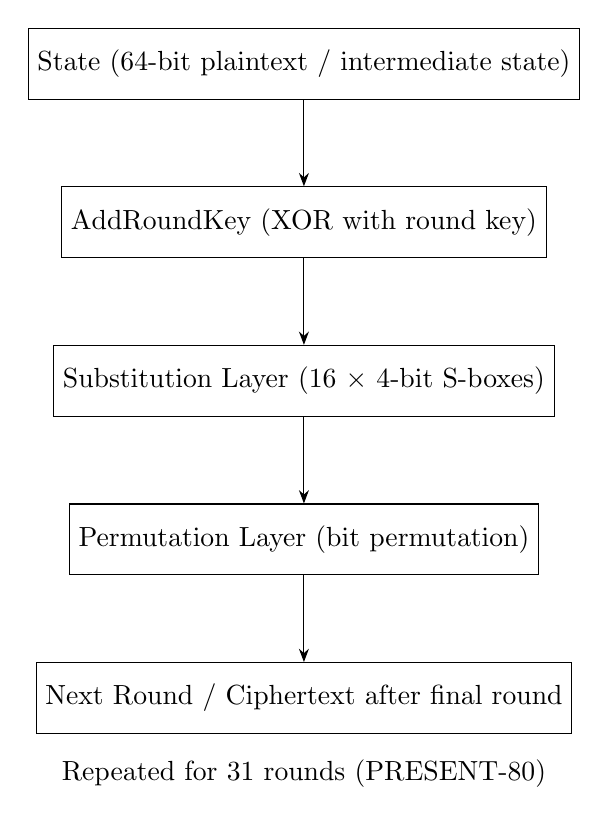
\begin{tikzpicture}[
            node distance=1.1cm,
            box/.style={draw, minimum width=5cm, minimum height=0.9cm, align=center},
            >=Stealth
        ]
        \node[box] (in) {State (64-bit plaintext / intermediate state)};
        \node[box, below=of in] (kadd) {AddRoundKey (XOR with round key)};
        \node[box, below=of kadd] (sbox) {Substitution Layer (16 $\times$ 4-bit S-boxes)};
        \node[box, below=of sbox] (perm) {Permutation Layer (bit permutation)};
        \node[box, below=of perm] (next) {Next Round / Ciphertext after final round};

        \draw[->] (in) -- (kadd);
        \draw[->] (kadd) -- (sbox);
        \draw[->] (sbox) -- (perm);
        \draw[->] (perm) -- (next);

        \node[below=0.2cm of next] {Repeated for 31 rounds (PRESENT-80)};
    \end{tikzpicture}
    \caption{Simplified round structure of the PRESENT block cipher.}
    \label{fig:present-round}
\end{figure}

\subsection*{High-Level Encryption Pseudocode}

\begin{algorithm}[H]
    \caption{PRESENT Encryption (High-Level)}
    \label{alg:present-encrypt}
    \begin{algorithmic}[1]
        \REQUIRE 64-bit plaintext state $S$, master key $K$
        \ENSURE 64-bit ciphertext $C$

        \STATE Generate round keys $\{K_1, K_2, \dots, K_{31}\}$ from $K$
        \FOR{$i = 1$ to $31$}
        \STATE $S \gets S \oplus K_i$ \hfill \COMMENT{AddRoundKey}
        \STATE $S \gets \textrm{SBoxLayer}(S)$
        \STATE $S \gets \textrm{PermutationLayer}(S)$
        \ENDFOR
        \STATE $C \gets S \oplus K_{32}$ \hfill \COMMENT{Final whitening (if used)}
        \RETURN $C$
    \end{algorithmic}
\end{algorithm}

The pseudocode above omits implementation details of the key schedule, S-box definitions, and bit
permutation, focusing instead on the round-level structure.

\section{SPECK}

\subsection*{Structure and Design Goals}

SPECK is a family of lightweight block ciphers optimized for software using an ARX
(Add–Rotate–XOR) design~\cite{beaulieu2015simon}. It uses a simple Feistel-like structure
with word-wise additions modulo $2^n$, rotations, and XOR operations. This makes SPECK
highly efficient on microcontrollers, particularly in software-only environments.

\subsection*{Round Function Diagram}

\begin{figure}[H]
    \centering
    \begin{tikzpicture}[
            node distance=1.3cm,
            box/.style={draw, minimum width=3.3cm, minimum height=0.9cm, align=center},
            >=Stealth
        ]
        \node[box] (in) {$L, R$ (two $n$-bit words)};
        \node[box, below=of in] (rotl) {$L' = \text{ROR}(L, \alpha)$};
        \node[box, below=of rotl] (add) {$L'' = (L' + R) \bmod 2^n$};
        \node[box, below=of add] (kadd) {$L''' = L'' \oplus K_i$};
        \node[box, below=of kadd] (rotr) {$R' = \text{ROL}(R, \beta)$};
        \node[box, below=of rotr] (out) {$L \gets L''', \; R \gets R'$};

        \draw[->] (in) -- (rotl);
        \draw[->] (rotl) -- (add);
        \draw[->] (add) -- (kadd);
        \draw[->] (kadd) -- (rotr);
        \draw[->] (rotr) -- (out);

        \node[below=0.2cm of out] {Repeated for a fixed number of rounds (e.g., 26 for SPECK-64/128).};
    \end{tikzpicture}
    \caption{Simplified round of the SPECK block cipher (ARX Feistel-like structure).}
    \label{fig:speck-round}
\end{figure}

\subsection*{High-Level Encryption Pseudocode}

\begin{algorithm}[H]
    \caption{SPECK Encryption (High-Level)}
    \label{alg:speck-encrypt}
    \begin{algorithmic}[1]
        \REQUIRE Two $n$-bit words $(L, R)$ as plaintext, round keys $\{K_0, \dots, K_{T-1}\}$
        \ENSURE Two $n$-bit words $(L, R)$ as ciphertext

        \FOR{$i = 0$ to $T-1$}
        \STATE $L \gets \textrm{ROR}(L, \alpha)$
        \STATE $L \gets (L + R) \bmod 2^n$
        \STATE $L \gets L \oplus K_i$
        \STATE $R \gets \textrm{ROL}(R, \beta)$
        \STATE $R \gets R \oplus L$
        \ENDFOR
        \RETURN $(L, R)$
    \end{algorithmic}
\end{algorithm}

Here, $\alpha$ and $\beta$ are rotation constants determined by the chosen SPECK variant (e.g., SPECK-64/128).

\section{ASCON}

\subsection*{Structure and Design Goals}

ASCON is a family of lightweight authenticated encryption and hashing algorithms based on
a permutation over a 320-bit internal state~\cite{dobraunig2016ascon,nist2023lwc}. The
state is typically viewed as five 64-bit words. ASCON uses a sponge-duplex construction,
where data is absorbed into part of the state (the rate), interleaved with permutation
calls, and then ciphertext and authentication tags are produced by squeezing from the same state.

\subsection*{Sponge-Duplex Overview}

\begin{figure}[H]
    \centering
    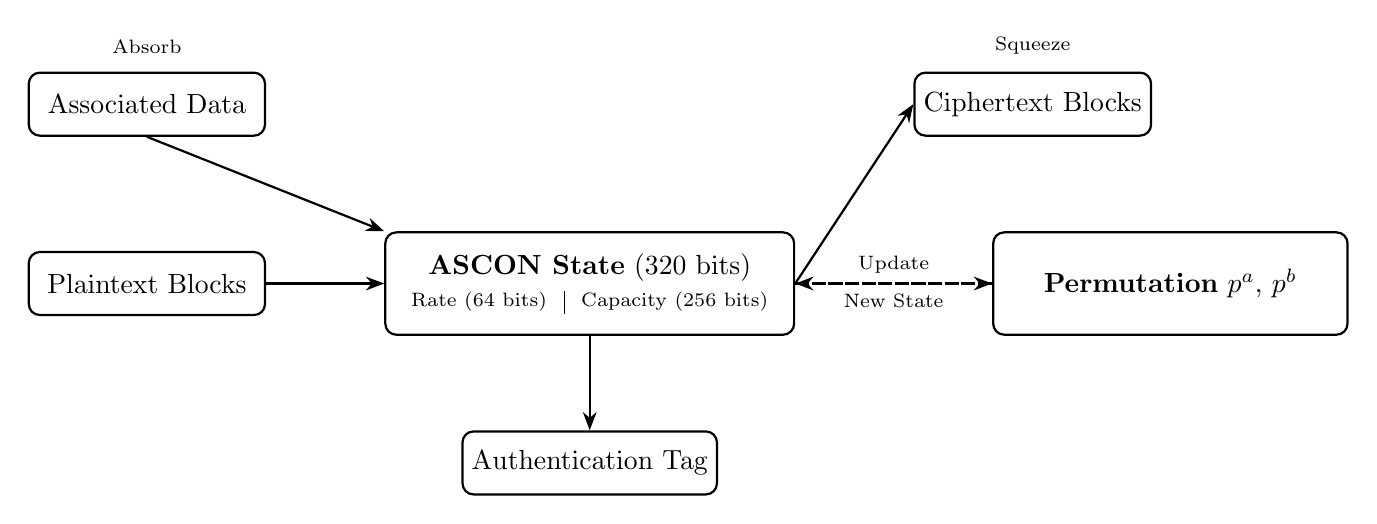
\begin{tikzpicture}[
            box/.style={draw, rounded corners, thick, minimum width=4.5cm, minimum height=1.3cm, align=center},
            smallbox/.style={draw, rounded corners, thick, minimum width=3cm, minimum height=0.8cm, align=center},
            arrow/.style={->, thick, >=Stealth},
            node distance=1.2cm and 1.5cm
        ]

        \node[box] (state) {
            \textbf{ASCON State} (320 bits)\\
            \scriptsize
            \begin{tabular}{c|c}
                Rate (64 bits) & Capacity (256 bits) \\
            \end{tabular}
        };

        \node[smallbox, above left=of state] (ad) {Associated Data};
        \node[smallbox, left=of state] (pt) {Plaintext Blocks};

        \node[smallbox, above right=of state] (ct) {Ciphertext Blocks};
        \node[smallbox, below=of state] (tag) {Authentication Tag};

        \node[box, right=2.5cm of state] (perm) {\textbf{Permutation} $p^a$, $p^b$};

        \draw[arrow, dashed] (state.east) -- node[above] {\scriptsize Update} (perm.west);
        \draw[arrow, dashed] (perm.west) -- node[below] {\scriptsize New State} (state.east);

        \draw[arrow] (ad.south) -- (state.north west);
        \draw[arrow] (pt.east) -- (state.west);
        \draw[arrow] (state.east) -- (ct.west);
        \draw[arrow] (state.south) -- (tag.north);

        \node[above=0.1cm of ad] {\scriptsize Absorb};
        \node[above=0.1cm of ct] {\scriptsize Squeeze};

    \end{tikzpicture}
    \caption{ASCON authenticated encryption using a sponge-duplex structure.}
    \label{fig:ascon_sponge_modern}
\end{figure}

\subsection*{High-Level AEAD Pseudocode}

\begin{algorithm}[H]
    \caption{ASCON AEAD Encryption (High-Level)}
    \label{alg:ascon-aead}
    \begin{algorithmic}[1]
        \REQUIRE Key $K$, nonce $N$, associated data $A$, plaintext $P$
        \ENSURE Ciphertext $C$, authentication tag $T$

        \STATE Initialize 320-bit state with $K$, $N$, and IV
        \STATE Apply initial permutation $p$

        \STATE \textbf{Absorb associated data}:
        \FOR{each block $A_i$ of $A$}
        \STATE Absorb $A_i$ into the rate portion of the state
        \STATE Apply permutation $p$
        \ENDFOR

        \STATE \textbf{Encrypt plaintext and produce ciphertext}:
        \FOR{each block $P_i$ of $P$}
        \STATE Absorb $P_i$ into the rate portion of the state
        \STATE $C_i \gets$ part of the state (rate) XOR $P_i$
        \STATE Apply permutation $p$
        \ENDFOR

        \STATE \textbf{Finalize and generate tag}:
        \STATE Inject key material into the state
        \STATE Apply final permutation $p$
        \STATE Derive tag $T$ from part of the state

        \RETURN $(C, T)$
    \end{algorithmic}
\end{algorithm}

This pseudocode abstracts away implementation-specific details, such as padding rules, exact
rate/capacity split, and permutation round counts, but it captures the main structure of ASCON’s
authenticated-encryption mode.

\chapter{Proposed Comparative Framework and Methodology}

This chapter presents the methodology used to evaluate the lightweight cryptographic
algorithms—PRESENT, SPECK, and ASCON—on an embedded platform. The objective is to enable a
fair, reproducible, and practically feasible comparison using software-based instrumentation
on the Raspberry Pi Pico~\cite{raspberry2021pico}. The methodology covers performance
measurements, memory analysis, security considerations, and the rationale behind algorithm selection.

\section{Evaluation Criteria}

Lightweight cryptographic algorithms must be assessed along dimensions relevant to constrained
devices. The evaluation criteria integrate quantitative measurements from Rust implementations
with qualitative analysis based on cryptographic literature.

\subsection{Performance Metrics}

Performance evaluation focuses on execution efficiency on the ARM Cortex-M0+ microcontroller.

\subsubsection*{Execution Time}
Execution time measurements include:
\begin{itemize}
    \item Key schedule generation,
    \item Single-block encryption and decryption,
    \item Full-message encryption for 64~B, 256~B, and 1024~B inputs.
\end{itemize}

Timing measurements utilize the hardware timer available on the Raspberry Pi Pico via the
\texttt{rp2040-hal} crate. Cycle counts are calculated as:
\[
    \textit{cycles} = \textit{time in seconds} \times 133\text{ MHz}.
\]

\subsubsection*{Cycles Per Byte (CPB)}
CPB, a platform-independent indicator of efficiency, is computed as:
\[
    \textit{CPB} = \frac{\textit{total cycles}}{\textit{total bytes processed}}.
\]

\subsubsection*{Memory Utilization}
Memory analysis records:
\begin{itemize}
    \item \textbf{ROM footprint}: compiled binary size (\texttt{cargo size --release}),
    \item \textbf{Static RAM usage}: ELF metadata (\texttt{.bss} and \texttt{.data} sections),
    \item \textbf{Working RAM}: estimated from internal state, S-boxes, and buffers.
\end{itemize}

\subsubsection*{Throughput}
Throughput (bytes/s) is measured by encrypting buffers of fixed sizes:
\[
    \textit{throughput} = \frac{\textit{bytes processed}}{\textit{time}}.
\]
This metric highlights scaling behavior, particularly for ASCON’s authenticated mode.

\subsection{Security Metrics}

Security analysis is based on literature, focusing on theoretical strength and resilience
against practical attacks.

\subsubsection*{Security Level}
Comparison includes:
\begin{itemize}
    \item Key sizes (80-bit, 128-bit),
    \item Block sizes and internal state dimensions,
    \item Expected brute-force resistance.
\end{itemize}

\subsubsection*{Cryptanalytic Resistance}
The study summarizes known attacks, including differential and linear cryptanalysis,
meet-in-the-middle attacks, algebraic attacks, and rotational attacks (notably relevant
for ARX-based ciphers such as SPECK).

\subsubsection*{Structural Robustness}
A structural comparison evaluates:
\begin{itemize}
    \item PRESENT’s S-box and bit-permutation layer,
    \item SPECK’s ARX-based Feistel structure,
    \item ASCON’s sponge-based permutation.
\end{itemize}

\section{Algorithm Selection}

The selected algorithms represent diverse lightweight design approaches and are practical
for implementation on the Raspberry Pi Pico.

\subsection*{PRESENT}
A hardware-oriented SPN cipher standardized in ISO/IEC 29192-2. Its small hardware footprint
makes it a representative lightweight cipher for constrained devices.

\subsection*{SPECK}
A software-optimized ARX cipher offering high speed, low RAM usage, and compact code size.
It maps efficiently onto the Pico’s Cortex-M0+ instruction set.

\subsection*{ASCON}
The NIST Lightweight Cryptography Standard (2023), providing authenticated encryption with
balanced performance in hardware and software.

Together, these algorithms provide varied design philosophies while keeping the project scope manageable.

\section{Implementation Plan}

All experiments are conducted using Rust on the Raspberry Pi Pico to ensure practical
relevance and feasibility within the project timeline.

\subsection{Software and Hardware Environment}

\begin{itemize}
    \item \textbf{Hardware}: Raspberry Pi Pico (ARM Cortex-M0+, 133\,MHz, 264\,KB SRAM, 2\,MB Flash),
    \item \textbf{Language}: Rust (\texttt{no\_std} environment for embedded targets),
    \item \textbf{Tools}: \texttt{rp2040-hal}, \texttt{probe-rs}, \texttt{cargo-embed},
    \item \textbf{Build Profile}: Release mode with LTO and size optimization.
\end{itemize}

\subsection{Performance Measurement Procedure}

\begin{itemize}
    \item Use the hardware timer for cycle-accurate timing,
    \item Average results over at least 1000 iterations,
    \item Measure both single-block and multi-block performance,
    \item For ASCON, evaluate initialization, associated-data processing, encryption, and tag generation.
\end{itemize}

\subsection{Memory Profiling Procedure}

\begin{itemize}
    \item Extract ROM and RAM usage from build artifacts,
    \item Identify memory-heavy components such as S-box tables or state buffers.
\end{itemize}

\section{Summary of Methodology}

This methodology enables a fair and meaningful comparison of PRESENT, SPECK, and ASCON
within the context of lightweight cryptography for constrained embedded systems.

\chapter{Expected Results and Discussion}

This chapter outlines the expected outcomes from the implementation and benchmarking of the PRESENT, SPECK, and ASCON algorithms on the Raspberry Pi Pico platform. Since the actual experimental results will be obtained during the implementation phase, this chapter provides a discussion of anticipated trends based on published literature and the design characteristics of each algorithm.

\section{Expected Performance Results}

Algorithm performance on constrained microcontrollers is influenced by internal structure, operation complexity, and memory requirements. Based on published evaluations and design characteristics, the following performance trends are anticipated.

\subsection{Execution Time}

\begin{itemize}
    \item \textbf{SPECK} is expected to provide the fastest execution time. Its ARX-based structure maps efficiently to the Cortex-M0+ instruction set, resulting in low cycles per round.
    \item \textbf{PRESENT} is expected to exhibit slower performance due to S-box lookups and bit-permutation operations that introduce software overhead.
    \item \textbf{ASCON} is expected to perform between PRESENT and SPECK. Its larger internal state (320 bits) and authenticated encryption requirements increase computational cost.
\end{itemize}

These trends should be observable in timing and cycle-per-byte (CPB) measurements.

\subsection{Throughput}

\begin{itemize}
    \item \textbf{SPECK} is expected to achieve the highest throughput across different input sizes due to its streamlined round function.
    \item \textbf{ASCON} may demonstrate improved throughput for longer messages, as its initialization cost becomes amortized over larger inputs.
    \item \textbf{PRESENT} is expected to provide the lowest throughput due to its bitwise round transformations.
\end{itemize}

\[
    \text{Throughput (expected): SPECK} > \text{ASCON} > \text{PRESENT}.
\]

\section{Expected Memory Utilization}

\textbf{ROM (Binary Size):}
SPECK is expected to require the smallest ROM footprint because it relies exclusively on simple arithmetic and bitwise operations. PRESENT may require additional storage for S-box tables, but should remain compact overall. ASCON is expected to have the highest ROM usage due to its larger state and more complex permutations.

\textbf{RAM Usage:}
PRESENT and SPECK are expected to use minimal static and working RAM. ASCON is expected to consume more RAM because it maintains a 320-bit internal state and additional temporary structures for authenticated encryption.

\[
    \text{RAM (expected): PRESENT} \approx \text{SPECK} < \text{ASCON}.
\]

\section{Expected Security Observations}

All three algorithms provide practical levels of security for lightweight cryptography, but their assurances differ:

\begin{itemize}
    \item \textbf{ASCON} offers the strongest modern security guarantees and was selected as the NIST Lightweight Cryptography Standard.
    \item \textbf{PRESENT-128} provides suitable margins for long-term embedded deployments, whereas PRESENT-80 is more appropriate for short-lifetime applications.
    \item \textbf{SPECK} maintains good cryptanalytic resistance but has tighter margins and continues to receive scrutiny due to its origins.
\end{itemize}

\section{Illustrative Result Tables}

The following table is a placeholder that will be populated with empirical results in the final report.

\begin{table}[H]
    \centering
    \begin{tabular}{lccc}
        \hline
        \textbf{Algorithm} & \textbf{Expected Speed} & \textbf{Expected ROM} & \textbf{Expected RAM} \\
        \hline
        PRESENT            & Medium                  & Medium                & Low                   \\
        SPECK              & High                    & Low                   & Low                   \\
        ASCON              & Medium                  & High                  & Medium                \\
        \hline
    \end{tabular}
    \caption{Anticipated performance and memory-efficiency trends.}
    \label{tab:expected-trends}
\end{table}

\section{Discussion}

Based on expected trends, SPECK is anticipated to deliver the best performance in software, making it suitable for real-time microcontroller applications. PRESENT, while slower, provides exceptional compactness that benefits low-cost hardware platforms. ASCON is expected to deliver a favorable balance of modern security and acceptable performance, particularly for systems requiring authenticated encryption.

These predictions reinforce a core principle of lightweight cryptography: different algorithms are optimized for different constraints, and therefore no single design dominates across all dimensions.

The empirical results obtained during experimentation will validate or refine these expectations and provide deeper insight into real-world suitability for embedded deployment.

\chapter{Conclusion and Future Work}

\section{Conclusion}

This study investigates lightweight cryptographic algorithms tailored for resource-constrained embedded platforms. A detailed literature review contextualizes the evolution of modern cryptography and highlights the emergence of lightweight approaches driven by IoT deployment challenges.

Three representative algorithms—PRESENT, SPECK, and ASCON—were selected to evaluate performance, memory efficiency, and theoretical security strength. The proposed methodology enables a structured comparison using Rust-based implementations on the Raspberry Pi Pico.

Expected trends suggest that SPECK will provide superior performance, PRESENT will offer minimal memory footprint, and ASCON will deliver strong modern security with functional completeness. Algorithm selection in embedded systems must therefore align with specific application needs and deployment constraints.

This report establishes a foundation for empirical benchmarking and provides methodological guidelines for further work.

\section{Future Work}

Future research can extend this study in the following directions:

\begin{itemize}
    \item \textbf{Energy consumption analysis}: Measuring power efficiency during encryption and decryption.
    \item \textbf{Evaluation of additional ciphers}: Including designs such as SIMON, GIFT, and PRINCE across multiple variants.
    \item \textbf{Hardware acceleration}: Assessing performance with cryptographic extensions or FPGA implementations.
    \item \textbf{Protocol integration}: Incorporating lightweight ciphers into IoT protocols such as MQTT, CoAP, or BLE.
    \item \textbf{Side-channel protection}: Investigating resilience to timing, power, and electromagnetic attacks.
    \item \textbf{Automation framework}: Developing reusable embedded benchmarking tools for timing, memory, and throughput profiling.
\end{itemize}

These directions will deepen the understanding of lightweight cryptographic design and facilitate secure IoT-system development.

\newpage
\bibliographystyle{plain}
\begin{thebibliography}{99}

    \bibitem{singh2000codebook}
    Simon Singh, \textit{The Code Book: The Science of Secrecy from Ancient Egypt to Quantum Cryptography}. Anchor Books, 2000.

    \bibitem{alkindi1987manuscript}
    Al-Kindi, ``Risāla fī Istikhrāj al-Mu'ammā'' (Manuscript on Deciphering Cryptographic Messages), circa 850 CE. In: M. Mrayati, Y. Alam, \textit{Series of Arabic Cryptography Manuscripts}, vol. 1, 1987.

    \bibitem{hodges2014turing}
    Andrew Hodges, \textit{Alan Turing: The Enigma}. Princeton University Press, 2014.

    \bibitem{nist2001aes}
    National Institute of Standards and Technology, ``Advanced Encryption Standard (AES),'' FIPS PUB 197, 2001.
    \url{https://nvlpubs.nist.gov/nistpubs/FIPS/NIST.FIPS.197.pdf}

    \bibitem{diffie1976new}
    W. Diffie and M. Hellman, ``New Directions in Cryptography,'' \textit{IEEE Transactions on Information Theory}, vol. 22, no. 6, pp. 644--654, 1976.
    \url{https://ee.stanford.edu/~hellman/publications/24.pdf}

    \bibitem{rivest1978method}
    R. Rivest, A. Shamir, and L. Adleman, ``A Method for Obtaining Digital Signatures and Public-Key Cryptosystems,'' \textit{Communications of the ACM}, vol. 21, no. 2, pp. 120--126, 1978.
    \url{https://people.csail.mit.edu/rivest/Rsapaper.pdf}

    \bibitem{bogdanov2007present}
    A. Bogdanov, L. R. Knudsen, G. Leander, C. Paar, A. Poschmann, M. J. B. Robshaw, Y. Seurin, and C. Vikkelsoe, ``PRESENT: An Ultra-Lightweight Block Cipher,'' in \textit{Proceedings of CHES 2007}, LNCS 4727, pp. 450--466, Springer, 2007.
    \url{https://link.springer.com/chapter/10.1007/978-3-540-74735-2_31}

    \bibitem{beaulieu2015simon}
    R. Beaulieu, D. Shors, J. Smith, S. Treatman-Clark, B. Weeks, and L. Wingers, ``The SIMON and SPECK Lightweight Block Ciphers,'' in \textit{Proceedings of the 52nd ACM/EDAC/IEEE Design Automation Conference (DAC)}, pp. 1--6, 2015.
    \url{https://eprint.iacr.org/2013/404.pdf}

    \bibitem{dobraunig2016ascon}
    C. Dobraunig, M. Eichlseder, F. Mendel, and M. Schläffer, ``ASCON v1.2: Lightweight Authenticated Encryption and Hashing,'' \textit{Journal of Cryptology}, vol. 34, no. 3, pp. 1--42, 2021.
    \url{https://ascon.iaik.tugraz.at/}

    \bibitem{nist2023lwc}
    National Institute of Standards and Technology, ``Lightweight Cryptography: ASCON,'' \textit{FIPS 203 (Draft)}, 2023.
    \url{https://csrc.nist.gov/pubs/fips/203/ipd}

    \bibitem{mckay2017nist}
    K. A. McKay and L. Bassham, ``Report on Lightweight Cryptography,'' NISTIR 8114, National Institute of Standards and Technology, 2017.
    \url{https://nvlpubs.nist.gov/nistpubs/ir/2017/NIST.IR.8114.pdf}

    \bibitem{guo2011photon}
    J. Guo, T. Peyrin, and A. Poschmann, ``The PHOTON Family of Lightweight Hash Functions,'' in \textit{Proceedings of CRYPTO 2011}, LNCS 6841, pp. 222--239, Springer, 2011.
    \url{https://link.springer.com/chapter/10.1007/978-3-642-22792-9_13}

    \bibitem{bogdanov2011spongent}
    A. Bogdanov, M. Knežević, G. Leander, D. Toz, K. Varıcı, and I. Verbauwhede, ``SPONGENT: A Lightweight Hash Function,'' in \textit{Proceedings of CHES 2011}, LNCS 6917, pp. 312--325, Springer, 2011.
    \url{https://link.springer.com/chapter/10.1007/978-3-642-23951-9_21}

    \bibitem{hell2007grain}
    M. Hell, T. Johansson, and W. Meier, ``Grain: A Stream Cipher for Constrained Environments,'' \textit{International Journal of Wireless and Mobile Computing}, vol. 2, no. 1, pp. 86--93, 2007.
    \url{https://dl.acm.org/doi/10.1504/IJWMC.2007.013798}

    \bibitem{canniere2008trivium}
    C. De Cannière and B. Preneel, ``Trivium,'' in \textit{New Stream Cipher Designs}, LNCS 4986, pp. 244--266, Springer, 2008.
    \url{https://link.springer.com/chapter/10.1007/978-3-540-68351-3_18}

    \bibitem{al2015iot}
    S. Al-Sarawi, M. Anbar, K. Alieyan, and M. Alzubaidi, ``Internet of Things (IoT) Communication Protocols: Review,'' in \textit{2017 8th International Conference on Information Technology (ICIT)}, 2017.
    \url{https://ieeexplore.ieee.org/document/8079928}

    \bibitem{raspberry2021pico}
    Raspberry Pi Foundation, ``Raspberry Pi Pico Datasheet,'' 2021.
    \url{https://datasheets.raspberrypi.com/pico/pico-datasheet.pdf}

    \bibitem{rustembedded2022}
    Rust Embedded Working Group, ``The Embedded Rust Book,'' 2022.
    \url{https://docs.rust-embedded.org/book/}

\end{thebibliography}

\end{document}
